Wir betrachten als erstes Voronoi Kanten zwischen Punkt $P$ und Strecke $s$ (siehe Abbildung~\ref{fig:ps}). Diese bestehen grundsätzlich aus drei Abschnitten. (i) und (iii) sind Strecken bzw. Strahlen. Es ist die Voronoi Kante zwischen dem Punkt $P$ und dem linken $A$ bzw. rechten Streckenende $B$. (ii) ist eine Parabel. Deren Form ist abhängig vom Abstand zwischen $P$ und $s$. In welchem Abschnitt $P$ liegt ist egal, die Zusammensetzung der Voronoi Kante bleibt gleich.

\begin{figure}[h!]
\begin{center}
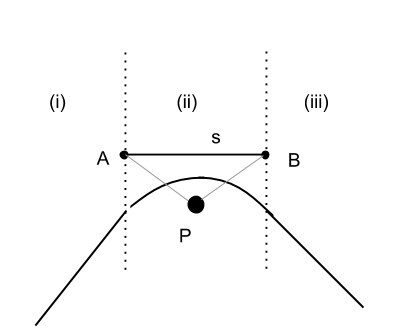
\includegraphics[width=7cm]{img/punkt-strecke.png}
\end{center}
\caption{Bisektor Punkt und Strecke}
\label{fig:ps}
\end{figure}

Betrachten wir nun die Bisektoren von zwei Strecken $s$ und $t$, dabei unterscheiden wir in (a) parallele Strecken und (b) nicht parallele Strecken.

\paragraph*{(a) parallele Strecken:}

\begin{itemize}
\item (1) $s$ und $t$ liegen auf einer Geraden (Spezialfall, siehe Abbildung~\ref{fig:sspc} )
\item (2) $s$ und $t$ "`überschneiden"' sich nicht (siehe Abbildung~\ref{fig:sspku})
\item (3) $s$ und $t$ "`überschneiden"' sich zum Teil oder ganz (siehe Abbildung~\ref{fig:sspu} und~\ref{fig:sspua})
\end{itemize}

Im Fall (2) und (3) entstehen fünf Abschnitte:\\
(i) Strecke: Bisektor der linkesten Punkte $A$ und $C$\\
(ii) Parabel: $s$ und $C$\\
(iii) Strecke: Gerade dazwischen\\
(iv) Parabel: $t$ und $B$\\
(v) Strecke: Bisektor der rechtesten Punkte $B$ und $D$\\

\begin{figure}[h!]
\begin{center}
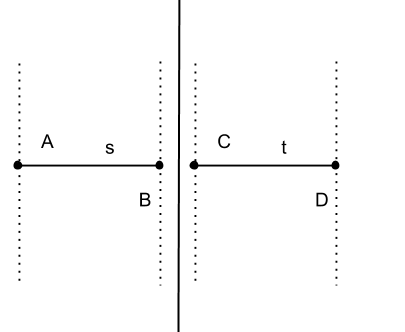
\includegraphics[width=7cm]{img/ssp1.png}
\end{center}
\caption{(1) Bisektor von zwei parallelen Strecken, die auf der gleichen Gerade liegen.}
\label{fig:sspc}
\end{figure}

\begin{figure}[h!]
\begin{center}
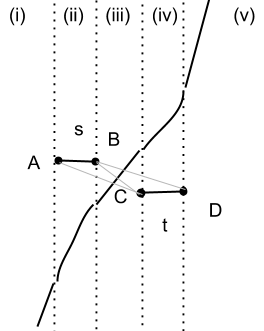
\includegraphics[width=5cm]{img/ssp2.png}
\end{center}
\caption{(2) Bisektor von zwei parallelen Strecken, keine Überschneidung.}
\label{fig:sspku}
\end{figure}

\begin{figure}[h!]
\begin{center}
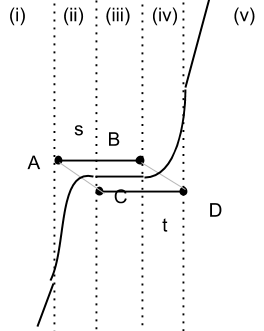
\includegraphics[width=5cm]{img/ss3.png}
\end{center}
\caption{(3) Bisektor von zwei parallelen Strecken, Überschneidung.}
\label{fig:sspu}
\end{figure}

\begin{figure}[h]
\begin{center}
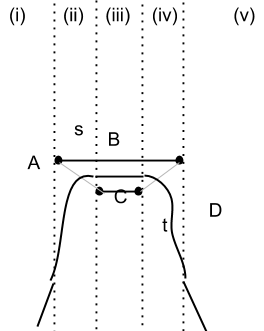
\includegraphics[width=5cm]{img/ss4.png}
\end{center}
\caption{(3) Bisektor von zwei parallelen Strecken, komplett innerhalb.}
\label{fig:sspua}
\end{figure}

\newpage

\paragraph*{(b) nicht parallele Strecken}

\begin{itemize}
\item (1) $s$ und $t$ "`überschneiden"' sich nicht
\item (2) $s$ und $t$ "`überschneiden"' sich zum Teil oder ganz
\end{itemize}

Hier entstehen im Fall (1) vier Abschnitte (siehe Abbildung~\ref{fig:ssnpku} ), im Fall (2) sieben Abschnitte (siehe Abbildung~\ref{fig:ssnpu}):\\

Fall (1): $s$ und $t$ "`überschneiden"' sich nicht\\
(i) Strecke\\
(ii) winkelhalbierende Strecke\\
(iii) Parabel\\
(iv) Strecke\\

\begin{figure}[h!]
\begin{center}
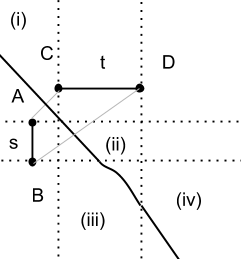
\includegraphics[width=5cm]{img/ssnpout.png}
\end{center}
\caption{(3) Bisektor von zwei nicht parallelen Strecken, keine Überschneidung.}
\label{fig:ssnpku}
\end{figure}

Fall (2): $s$ und $t$ "`überschneiden"' sich zum Teil oder ganz\\
(i) Parabel\\
(ii) 2$\times$winkelhalbierende Strecken\\
(iii) und (iv) Parabel\\
(v) Strecke\\
(vi) Parabel\\
(vii) Strecke\\

\begin{figure}[h!]
\begin{center}
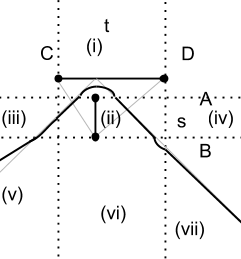
\includegraphics[width=5cm]{img/ssnpin.png}
\end{center}
\caption{(3) Bisektor von zwei nicht parallelen Strecken, mit Überschneidung.}
\label{fig:ssnpu}
\end{figure}

\paragraph*{Anzahl der Ecken, Kanten und Zellen} Die Anzahl der Zellen entspricht der Anzahl der Strecken $n$. Ein Bisektor zwischen zwei Strecken besteht höchstens aus 7 Abschnitten, d.h aus 6 Knoten ...